\section{Explicit Triangulations}
\label{sec:trias}


For small grids, one can enumerate all unimodular triangulations by
the reverse search algorithm 
sketched in Section~\ref{sec:values}. For
larger grids, it is desirable to obtain from the huge set of
unimodular triangulations ``random'' ones. There are ways to produce
them, however, in most cases the probability distribution from which
they are chosen is unknown.

\subsection{Generating Random Triangulations}
\label{subsec:rw}
A standard way to compute complex random objects such as triangulations
is to set up a random walk. In our case of unimodular triangulations
of $P_{m,n}$ the method is described easily: First one determines any
starting triangulation~$\mathcal{T}$ of $P_{m,n}$. Then, the following
operation is performed $\tau$ times: Choose one of the (inner) edges
of~$\mathcal{T}$ uniformly at random; if this edge is flippable (see
Section~\ref{sec:values}), then with probability $\frac12$ the current
triangulation $\mathcal{T}$ is replaced by the one obtained
from it by flipping that edge.

As the flip graph of the triangulations is connected (see
Section~\ref{sec:values}), it follows from general principles that,
with $\tau$ tending to infinity, the probability distribution defined by
the output of this algorithm converges to the uniform distribution
(with respect to the ``total variation distance''); see, e.g., Jerrum
and Sinclair~\cite{JerrumSinclair} or Behrends~\cite{Behrends-MarkovChains}.
Unfortunately, not much is known about the speed of convergence of the
distribution. In particular, for general~$m$ and~$n$ it is not known
whether there is a polynomial bound (in $n+m+\varepsilon^{-1}$) on the number~$\tau$
of steps needed to guarantee that the total variation distance between
the produced and the uniform distribution is at most~$\varepsilon$ (i.e.,
if the associated Markov chain is \emph{rapidly mixing}).  The only
exception is the case~$m=1$: Here it follows from results of
Felsner and Wernisch~\cite{FelsnerWernisch} that the Markov chain is
indeed rapidly mixing.

Despite this lack of knowledge on the distribution of the output of
the  random walk algorithm, one still can use it in order to produce
examples of ``interesting'' triangulations.

\subsection{Empirical Results}

For each $n\in\{10,\dots,20\}$, Meyer~\cite{Meyer} generated~$1000$
random unimodular triangulations of $P_{n,n}$ by running the random
walk described in Subsection~\ref{subsec:rw} $10^9$ steps, recording
every $10^6$th triangulation; see Table~\ref{tab:large}.
\begin{table}[ht]
  \centering
  \begin{tabular}{cccc}
    \hline
    $m\times n$ &
    \multicolumn{1}{c}{irregularity} & 
    \multicolumn{1}{c}{max. edge length} & 
    \multicolumn{1}{c}{av. edge length} \\
    \hline
    $10\times 10$ & .355 & 5.538 & 1.614 \\
    $11\times 11$ & .435 & 5.843 & 1.630 \\
    $12\times 12$ & .559 & 6.118 & 1.645 \\
    $13\times 13$ & .696 & 6.397 & 1.659 \\
    $14\times 14$ & .782 & 6.650 & 1.670 \\
    $15\times 15$ & .875 & 6.911 & 1.681 \\
    $16\times 16$ & .927 & 7.151 & 1.690 \\
    $17\times 17$ & .965 & 7.391 & 1.700 \\
    $18\times 18$ & .971 & 7.618 & 1.708 \\
    $19\times 19$ & .992 & 7.821 & 1.713 \\
    $20\times 20$ & .997 & 8.060 & 1.723 \\
    \hline
  \end{tabular}
  \caption{Results for random unimodular triangulations of large grids. The first
  column shows the (empirical) probability of irregularity, the
  second and third columns contain the (empirical) expected values of
  the maximal and the average edge length.}
  \label{tab:large}
\end{table}

The results  support the conjecture that, for~$n$ tending to
infinity, a random unimodular triangulation of $P_{n,n}$ is irregular
with probablity one. A second observation is that the (expected value)
of the average length of an edge in a random triangulation seems to
grow very slowly with~$n$. 

\subsection{Obstructions to Regularity}

All figures shown below have been produced by Meyer~\cite{Meyer}, who
implemented procedures for checking regularity by solving linear
programs using the \cplex\ library.

Proposition~\ref{prop:fregm12} shows that $P_{2,n}$ has only regular
triangulations.  The grid $P_{3,3}$ has precisely the following four
(pairwise congruent) irregular unimodular triangulations.
\begin{center}
  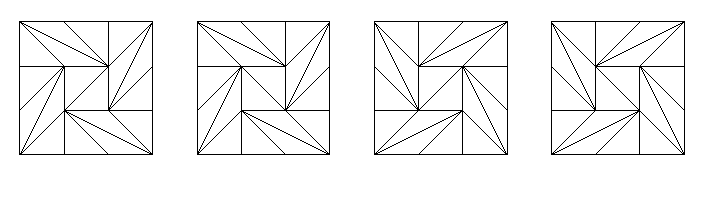
\includegraphics[width=.9\textwidth]{fig3x3irr_mod.ps}
\end{center}

When trying to understand the reasons for irregularity, it seems
useful to consider (smallest) forbidden patterns for regular
triangulations.  Let~$\mathcal{T}$ be a set of unimodular triangles of
$P_{m,n}$ (such that any two of them intersect in a common face).  We
denote by $S\subset P_{m,n}$ the set of all grid points covered by triangles
in~$\mathcal{T}$. The set~$\mathcal{T}$ is called \emph{regular} if
there is a height function $h:S\longrightarrow\R$ such that for each
triangle $\Delta\in\mathcal{T}$, all $h$-lifted points in 
$S{\setminus}\Delta$ lie strictly above the affine hull of the $h$-lifting
of~$\Delta$.  A subset of~$\mathcal{T}$ is called a 
\emph{minimal irregular configuration} if it is not regular, but all its proper
subsets are regular. Clearly, a regular unimodular triangulation of
$P_{m,n}$ cannot contain any minimal irregular configuration.

Examples for minimal irregular configurations of $P_{3,3}$ are the
following:
\begin{center}
  
\includegraphics[width=.9\textwidth]{fig3x3mic_mod.ps}
\end{center}

Already for $P_{3,4}$ many other minimal irregular
configurations occur; some are depicted here:
\begin{center}
  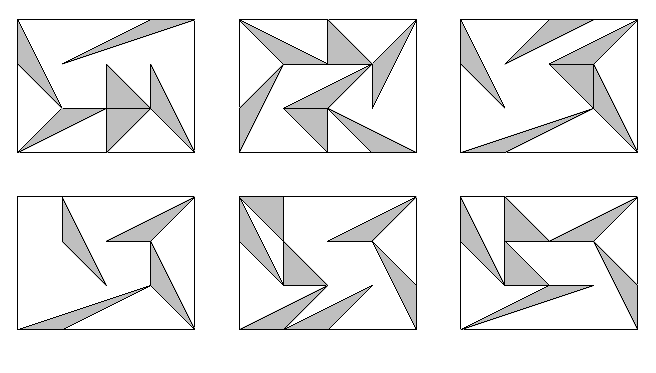
\includegraphics[width=.9\textwidth]{fig3x4mic_mod.ps}
\end{center}

While these figures still have some similarities with the nice
``whirlpools''
ones for $P_{3,3}$, the picture gets more and more complicated with
growing grid sizes, as the following examples demonstrate:

\begin{center}
  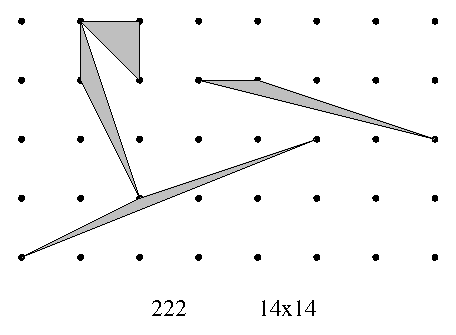
\includegraphics[width=.4\textwidth,bb=0 25 204 145,clip]{222.14_mod.eps}\hspace{.1\textwidth}%
  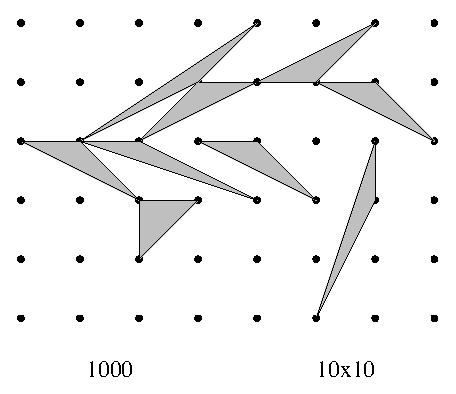
\includegraphics[width=.4\textwidth,bb=0 25 204 173,clip]{1000.10_mod.eps}  
\end{center}

\medskip
\begin{center}
  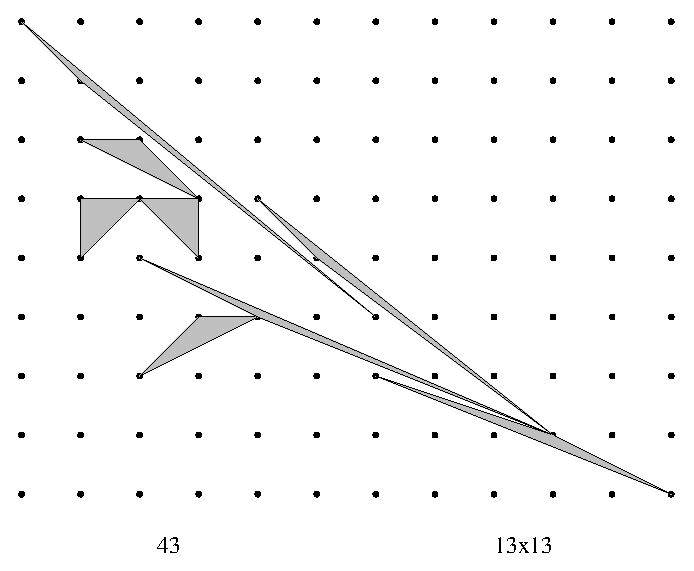
\includegraphics[width=.5\textwidth,bb=0 25 318 259,clip]{43.13_mod.eps}
\end{center}

Viewing these figures, it seems unlikely that one can find any compact
characterization of regularity for unimodular triangulations of
$P_{m,n}$ in terms of forbidden substructures.

We close our zoo of ``explicit triangulations'' with some pairs of
triangulations, found by Meyer's implementation of the random walk.
In each of the figures, the left triangulation is regular, but the right one is
not, although it can be obtained from the left one by flipping just
one edge (drawn bold in the upper left and in the lower right corner,
respectively). For both irregular triangulations, a minimal irregular
configuration contained in it is depicted as well.

\begin{center}
  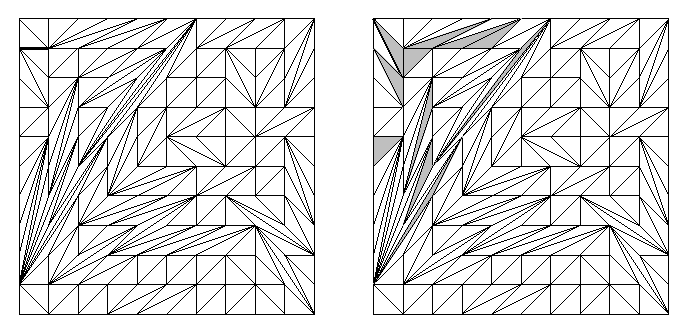
\includegraphics[width=.9\textwidth]{356357regirr_mod.eps}
\end{center}
\begin{center}
  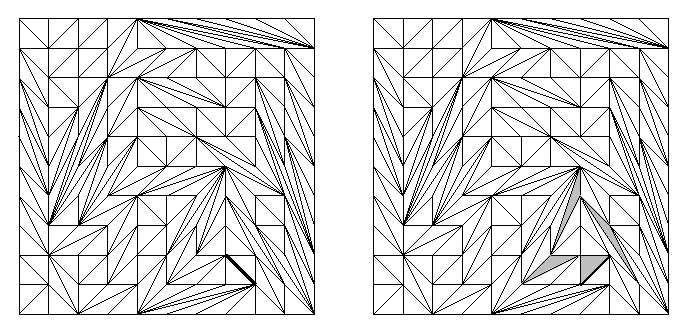
\includegraphics[width=.9\textwidth]{7576regirr_mod.eps}
\end{center}



%%% Local Variables:
%%% mode: latex
%%% TeX-master: "bcc_ct"
%%% End:
